\documentclass[
]{jss}

\usepackage[utf8]{inputenc}

\author{
Hanne Oberman\\Utrecht University \And Johanna Munoz Avila\\University
Medical Center Utrecht \AND Valentijn de Jong\\University Medical
Center Utrecht \And Gerko Vink\\Utrecht University \AND Thomas
Debray\\University Medical Center Utrecht
}
\title{Imputation of Incomplete Multilevel Data with \pkg{mice}}

\Plainauthor{Hanne Oberman, Johanna Munoz Avila, Valentijn de
Jong, Gerko Vink, Thomas Debray}
\Plaintitle{Imputation of Incomplete Multilevel Data with mice}
\Shorttitle{Multilevel \pkg{mice}}


\Abstract{
Multilevel data is not spared the ubiquitous problem of missing
information. This is a tutorial paper on imputing incomplete multilevel
data with \pkg{mice}. Including methods for ignorable and non-ignorable
missingness. Footnotes in the current version show work in
progress/under construction. The last section is not part of the
manuscript, but purely for reminders.
}

\Keywords{missing
data, multilevel, clustering, \pkg{mice}, \proglang{R}}
\Plainkeywords{missing data, multilevel, clustering, mice, R}

%% publication information
%% \Volume{50}
%% \Issue{9}
%% \Month{June}
%% \Year{2012}
%% \Submitdate{}
%% \Acceptdate{2012-06-04}

\Address{
    Hanne Oberman\\
    Utrecht University\\
    Padualaan 14\\
3584 CH Utrecht\\
  E-mail: \email{h.i.oberman@uu.nl}\\
  URL: \url{https://hanneoberman.github.io/}\\~\\
          }


% tightlist command for lists without linebreak
\providecommand{\tightlist}{%
  \setlength{\itemsep}{0pt}\setlength{\parskip}{0pt}}



\usepackage{graphicx}
\usepackage{mathtools}
\usepackage{ulem}

\usepackage{amsmath}

\begin{document}



\hypertarget{introduction}{%
\section{Introduction}\label{introduction}}

In many contemporary data analysis efforts, some form of hierarchical or
clustered structure is recorded. For example, students clustered within
schools, or patients clustered within studies in individual patient data
meta-analyses. Analyzing such multilevel data requires specialized
techniques that take the clustered structure into account, since
ignoring it may be harmful to the statistical inferences and can yield
biased results. Imagine a case where cross-level interactions between
unit-level variables and cluster-level variables are present. The
cluster to which a unit belongs may then influence the unit-level
observations--and vice versa for each of the units that make up the
cluster \citep{hox17}. These relations can and should be taken into
account when developing analysis models for multilevel data for the
simple reason that groups of observations share some common variance.

The variability due to clustering is often measured by means of the
intra-class coefficient (ICC). The ICC can be seen as the percentage of
variance that can be attributed to the cluster-level, where a high ICC
would indicate that a lot of variability is due to the cluster
structure. Multilevel models typically accommodate for this variability
by including separate intercepts for each cluster. Such fixed effects
relieve the restriction imposed by single-level models: equal group
means across clusters. Additionally, models may include random effects
of predictors across clusters, and random error terms (heterogeneous
residual error variances; see e.g. \citet{hox17} and \citet{jong21}).
There are many names for models that take clustering into account. Some
popular examples are `multilevel models', `hierarchical models', `mixed
effect models' and `random effect models'.

\hypertarget{incomplete-multilevel-data}{%
\subsection{Incomplete multilevel
data}\label{incomplete-multilevel-data}}

\begin{CodeChunk}
\begin{figure}

{\centering 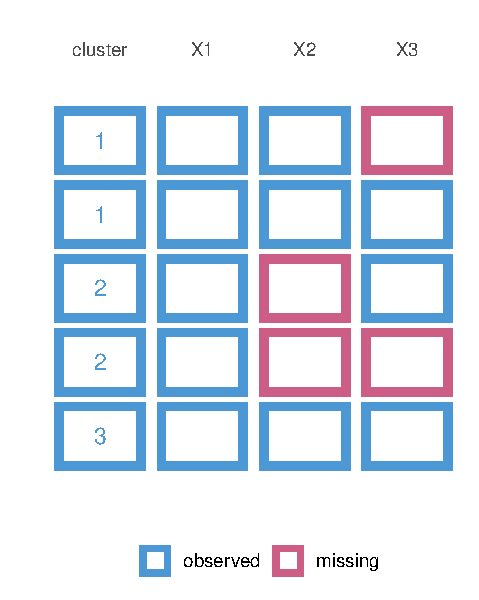
\includegraphics{Manuscript_files/figure-latex/patterns-1} 

}

\caption[Missingness in multilevel data]{Missingness in multilevel data}\label{fig:patterns}
\end{figure}
\end{CodeChunk}

The process of analyzing multilevel data is further complicated when not
all data entries are observed. Just as with single level data,
missingness may occur at the unit level. But with multiple levels of
data comes the potential for clustered missingness. Missingness in
multilevel data can therefore be categorized into two general patterns:
systematic missingness and sporadic missingness \citep{resc13}. We have
visualized the difference between these types of missingness in Figure
1. The figure shows an \(n \times p\) set
\(\mathbf{X} = X_1, \dots, X_p\), with \(n\) units distributed over
\(N\) clusters, and \(p=3\) columns. Column \texttt{X1} is completely
observed. Column \texttt{X2} is systematically missing and column
\texttt{X3} is sporadically missing. Systematic missingness can be
further subdivided into unobserved constants (i.e., the same value
within clusters) and non-measured random variables (which may differ per
unit within clusters). In Figure 1, the former would imply that the
unobserved values for units 3 and 4 on column \texttt{X2} are identical.
With the latter, the values would differ. The optimal strategy for
dealing with the missingness may therefore depend on the observed
missing data pattern.

Another characteristic of the missing data to take into account in
analyses is the mechanism behind the missingness. Although the essence
of the true non-response mechanism may not be known, it can be inferred
or assumed to be one of the following:

\begin{itemize}
\tightlist
\item
  Missing Completely At Random (MCAR), where the probability to be
  missing is equal across all data entries;
\item
  Missing At Random (MAR), where the probability to be missing depends
  on observed information;
\item
  Missing Not At Random (MNAR), where the probability to be missing
  depends on unrecorded information, making the missingness
  non-ignorable \citep{rubi76, meng94}. Depending on the assumed
  missingness mechanism, missing data handling strategies may be more or
  less suitable, see e.g., \citet{yuce08} and \citet{hox15}.
\end{itemize}

Ignoring the missingness in analyses can be extremely harmful to
inferences. Complete case analysis (i.e., excluding all units with one
or more missing entries) can introduce bias in statistical inference and
lowers statistical power. Instead, the missingness should be
accommodated \emph{before} or \emph{within} the analysis of scientific
interest. Especially the former is very generic and popular and is
widely known as imputation. Imputing (i.e., filling in) the missing
values separates the missing data problem from the scientific problem:
missing data are replaced by plausible values whereafter the completed
data is analysed as if it were completely observed. The \proglang{R}
package \pkg{mice} has become the de-facto standard for imputation by
chained equations, which iteratively solves the missingness on a
variable-by-variable basis. \pkg{mice} is known to yield valid
inferences under many different missing data circumstances
\citep{buur18}. In this paper, we'll discuss how to use \pkg{mice} in
the context of multilevel data, under varying missing data mechanisms.

\hypertarget{aim-of-this-paper}{%
\subsection{Aim of this paper}\label{aim-of-this-paper}}

This papers serves as a tutorial for imputing incomplete multilevel data
with \pkg{mice}. We provide practical guidelines and code snippets for
different missing data situations. For reasons of brevity, we focus on
imputation by chained equations exclusively (although the alternative,
joint modeling imputation for multilevel data or \pkg{jomo}
\citet{jomo}, has been implemented in \pkg{mice} as well). Other useful
resources for the analysis of incomplete multilevel data include the
\proglang{R} packages \pkg{mitml}, \pkg{miceadds}, and \pkg{mdmb}, and
the empirical work by \citet{audi18} and \citet{grun18}. Note that this
tutorial paper assumes a basic level of knowledge on multilevel models.
We're providing an overview of implementations. It's up-to the reader to
decide which multilevel strategy suits their data. We won't go into
detail for the different methods (and equations). This paper is just a
software tutorial, so we'll keep it practical.

To illustrate how to impute incomplete multilevel data, we structure
this tutorial around three case studies:

\begin{itemize}
\tightlist
\item
  \texttt{mice::popmis} (simulated data on perceived popularity,
  \(n = 199\) pupils across \(N = 10\) classes, with univariate MAR
  missingness);
\item
  \texttt{GJRM::hiv} (simulated data on HIV diagnoses, \(n = 6,416\)
  patients across \(N = 9\) regions, with univariate MNAR missingness)
\item
  \texttt{metamisc::impact} (empirical data on traumatic brain injuries,
  \(n = 11,022\) patients across \(N = 15\) studies, without
  \texttt{NA}s).
\end{itemize}

In each case study we highlight one aspect of the imputation workflow.
With the \texttt{mice::popmis} data, we show different ways of designing
an imputation model and what happens if you misspecify this model. With
the \texttt{GJRM::hiv} data we extend the imputation model to include
Heckman-type selection-inclusion methods. And with the
\texttt{metamisc::impact} data we provide a example of multivariate
missingness in real-world data. For all case studies we discuss the
nature of the incomplete data, the imputation model(s), and evaluation
of the imputed data: A. Choose an analysis model (so the imputation
model will be compatible with the analyses); B. Evaluate the incomplete
data; C. Develop the imputation model(s); D. Impute the missingness; E.
Evaluate the imputations.

\hypertarget{how-not-to-impute-case-study-i-popularity}{%
\section{How (not) to impute (Case Study I:
Popularity)}\label{how-not-to-impute-case-study-i-popularity}}

\texttt{popNCR2} is a simulated dataset with pupils clustered in
classes, where the number of units \(n = 2000\), and the number of
clusters \(N = 100\), on 7 variables:

\begin{itemize}
\tightlist
\item
  \texttt{pupil} Pupil number within class,
\item
  \texttt{class} Class number,
\item
  \texttt{extrav} Pupil extraversion,
\item
  \texttt{sex} Pupil gender,
\item
  \texttt{texp} Teacher experience (years),
\item
  \texttt{popular} Pupil popularity,
\item
  \texttt{popteach} Teacher popularity.
\end{itemize}

\hypertarget{incomplete-data}{%
\subsubsection{Incomplete data}\label{incomplete-data}}

\begin{CodeChunk}
\begin{figure}

{\centering 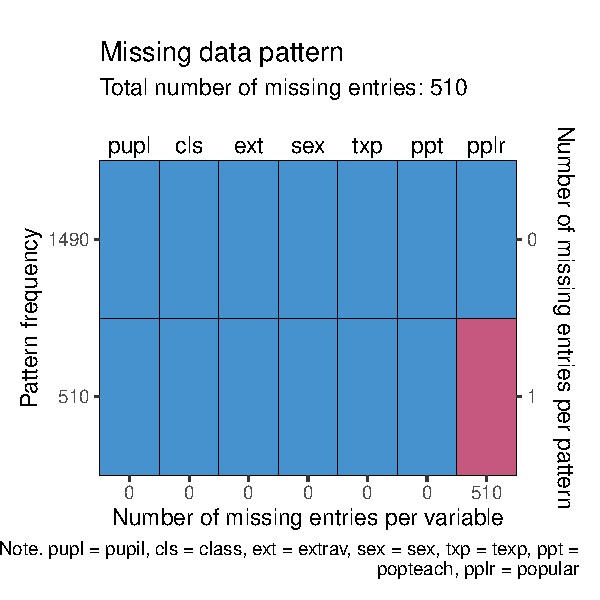
\includegraphics{Manuscript_files/figure-latex/pop_pat-1} 

}

\caption[Missing data pattern in the popularity data]{Missing data pattern in the popularity data}\label{fig:pop_pat}
\end{figure}
\end{CodeChunk}

The popularity data is created such that there are strong relations
between the incomplete variables and the clustering variable
\texttt{class}. We can express this using the intra-class correlation
(ICC). For \texttt{popular} the ICC is 0.4. For \texttt{popteach} it is
0.36. It would thus be wise to use multilevel modeling.

The missingness in this dataset is induced conform MAR and MNAR
mechanisms. The missing data pattern, Figure \ref{fig:pop_pat}, shows
that just one variable is incomplete \textbf{{[}the next part is not yet
updated to reflect this{]}}.

To develop the best imputation model, we need to know whether the
missingness in one variable depends on the observed values of other
variables. Visual inspection usually suffices. We'll highlight only two
variables to illustrate, but ideally one would inspect all relations.
The questions we'll ask are: `Does the missing data of \texttt{popular}
depend on \texttt{popteach}?' and `Does the missingness in teacher
popularity depend on pupil popularity?' We'll evaluate this by making a
histogram of \texttt{popteach} separately for the pupils with known
popularity and missing popularity, and the other way around.

In Figure \ref{fig:pop_dist} we see that the distribution for the
missing \texttt{popular} is further to the right than the distribution
for observed \texttt{popular}. This would indicate a right-tailed MAR
missingness. In fact, this is exactly what happens, because the
missingness in these data was created manually. Now, we've made it
observable by examining the relations between the missingness in popular
and the observed data in \texttt{popteach}. There is also a dependency
between the missingness in teacher popularity and pupil popularity. The
relation seems to be right-tailed as well.

\hypertarget{complete-case-analysis-not-recommended}{%
\subsubsection{Complete case analysis (not
recommended)}\label{complete-case-analysis-not-recommended}}

Complete case analysis ignores the observations with missingness
altogether, which may even introduce bias in MCAR situations.

\hypertarget{imputation-ignoring-the-cluster-variable-not-recommended}{%
\subsubsection{Imputation ignoring the cluster variable (not
recommended)}\label{imputation-ignoring-the-cluster-variable-not-recommended}}

The first imputation model that we'll use is likely to be invalid. In
this model, we ignore the multilevel structure of the data, despite the
high ICCs. This is purely to illustrate the effects of ignoring the
clustering in our imputation effort.

We'll use predictive mean matching to impute the continuous variables
and logistic regression to impute the binary variable \texttt{sex}. We
do not use the observation identifier \texttt{pupil} or cluster
identifier \texttt{class} as predictors to impute other variables.

\begin{CodeChunk}
\begin{CodeInput}
R> # dry run to get imputation parameters
R> ini <- mice(pop, maxit = 0)
R> 
R> # extract predictor matrix and adjust
R> pred <- ini$pred
R> pred[, c("class", "pupil")] <- 0
R> 
R> # impute the data, ignoring the cluster structure
R> imp_ignored <- mice(pop, maxit = 1, pred = pred, print = FALSE)
\end{CodeInput}
\end{CodeChunk}

\begin{CodeChunk}


\begin{center}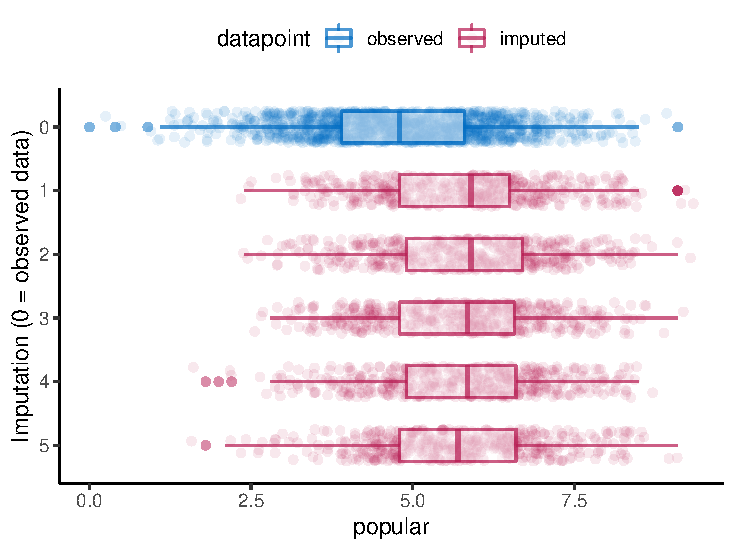
\includegraphics{Manuscript_files/figure-latex/pop_ignored_eval-1} \end{center}

\begin{CodeOutput}
      vars       CCA   ignored
1  popular 0.3989463 0.4235643
2 popteach 0.3605902 0.3605902
3     texp 1.0000000 1.0000000
\end{CodeOutput}
\end{CodeChunk}

As the original ICCs show, 100\% of the variance in \texttt{texp} can be
attributed to the clustering variable \texttt{class}. This tells us that
the multilevel structure of the data should be taken into account. If we
don't, we'll end up with incorrect imputations, biasing the effect of
the clusters towards zero.

We can also observe that the teacher experience increases slightly after
imputation. This is due to the MNAR missingness in \texttt{texp}. Higher
values for \texttt{texp} have a larger probability to be missing. This
may not a problem, however, if at least one pupil in each class has
teacher experience recorded, we can deductively impute the correct
(i.e.~true) value for every pupil in the class.

Add: Assumes exchangability between units.

\hypertarget{imputation-with-the-cluster-variable-as-predictor-not-recommended}{%
\subsubsection{Imputation with the cluster variable as predictor (not
recommended)}\label{imputation-with-the-cluster-variable-as-predictor-not-recommended}}

We'll now use \texttt{class} as a predictor to impute all other
variables. This is still not recommended practice, since it only works
under certain circumstances and results may be biased
\citep{drec15, ende16}. But at least, it includes some multilevel
aspect. This method is also called `fixed cluster imputation', and uses
N-1 indicator variables representing allocation of N clusters as a fixed
factor in the model \citep{reit06, ende2016}. Colloquially, this is
`multilevel imputation for dummies'.

Add: doesn't work with syst missing (only sporadically). There's some
pro's and con's. May not differ much if the number of clusters is low.

The more the random effects are of interest, the more you need ml
models.

\begin{CodeChunk}
\begin{CodeInput}
R> # adjust the predictor matrix
R> pred <- ini$pred 
R> pred[, "pupil"] <- 0
R> 
R> # impute the data, cluster as predictor
R> imp_predictor <- mice(pop, maxit = 1, pred = pred, print = FALSE)
\end{CodeInput}
\end{CodeChunk}

\begin{CodeChunk}


\begin{center}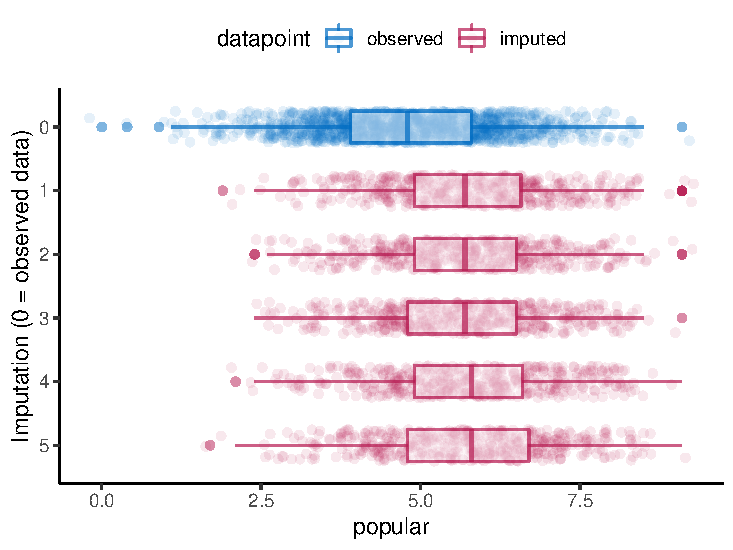
\includegraphics{Manuscript_files/figure-latex/pop_predictor_eval-1} \end{center}

\begin{CodeOutput}
      vars       CCA   ignored predictor
1  popular 0.3989463 0.4235643 0.3904372
2 popteach 0.3605902 0.3605902 0.3605902
3     texp 1.0000000 1.0000000 1.0000000
\end{CodeOutput}
\end{CodeChunk}

Now, we can clearly see that the imputed values of \texttt{texp} are
higher than the observed values, which is in line with right-tailed MAR.

The ICCs are way more in line with the ICCs in the incomplete data. But
this is a quick and dirty way of imputing multilevel data. We
\emph{should} be using a multilevel model.

\hypertarget{imputation-with-random-effects}{%
\subsubsection{Imputation with random
effects}\label{imputation-with-random-effects}}

With \texttt{2l.norm} we impute the outcome with a multilevel model
assuming random slopes for each variable in the imputation model and
homogeneous within-cluster variance.

\begin{CodeChunk}
\begin{CodeInput}
R> pred <- ini$pred
R> pred["popular", ] <- c(0, -2, 2, 2, 2, 0, 2) 
R> #-2 for the cluster variable, 2 for random effects
R> meth <- ini$meth
R> meth <- c("", "", "", "", "", "2l.norm", "")
R> imp_norm_2l <-
+   mice(
+     pop %>% mutate(class = as.integer(class)),
+     pred = pred,
+     meth = meth,
+     maxit = 1,
+     print = FALSE
+   )
\end{CodeInput}
\end{CodeChunk}

\begin{CodeChunk}


\begin{center}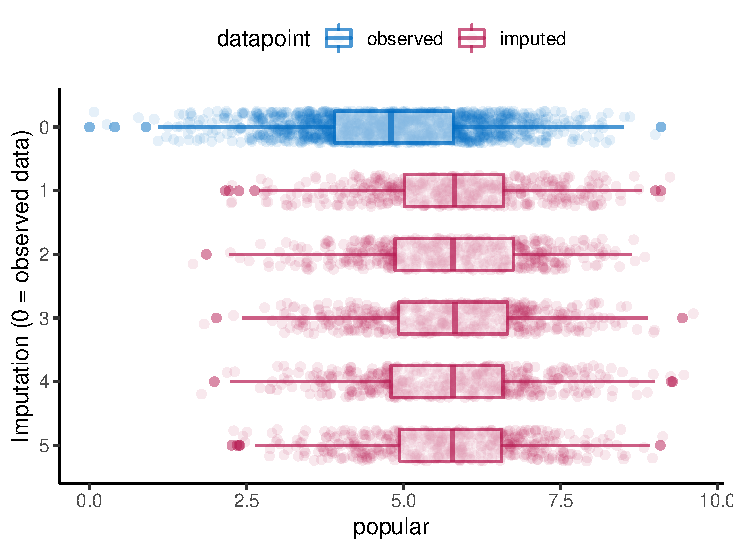
\includegraphics{Manuscript_files/figure-latex/pop_norm_eval-1} \end{center}

\begin{CodeOutput}
      vars       CCA   ignored predictor      norm
1  popular 0.3989463 0.4235643 0.3904372 0.4165006
2 popteach 0.3605902 0.3605902 0.3605902 0.3605902
3     texp 1.0000000 1.0000000 1.0000000 1.0000000
\end{CodeOutput}
\end{CodeChunk}

\hypertarget{imputation-with-random-effects-and-heterogeneity}{%
\subsubsection{Imputation with random effects and
heterogeneity}\label{imputation-with-random-effects-and-heterogeneity}}

This method assumes random slopes for each variable in the imputation
model. In contrast to \texttt{2l.norm} this method allows a
cluster-specific residual error variance.

\begin{CodeChunk}
\begin{CodeInput}
R> pred["popular", ] <- c(0, -2, 2, 2, 1, 0, 2)
R> meth <- c("", "", "", "", "", "2l.pan", "")
R> imp_pan_2l <-
+   mice(
+     pop %>% mutate(class = as.integer(class)),
+     pred = pred,
+     meth = meth,
+     maxit = 1,
+     print = FALSE
+   )
\end{CodeInput}
\end{CodeChunk}

\begin{CodeChunk}


\begin{center}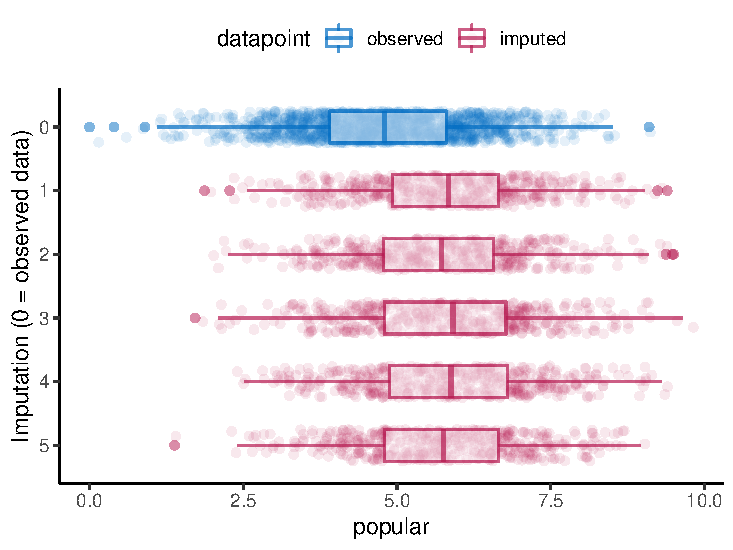
\includegraphics{Manuscript_files/figure-latex/pop_pan_eval-1} \end{center}

\begin{CodeOutput}
      vars       CCA   ignored predictor      norm       pan
1  popular 0.3989463 0.4235643 0.3904372 0.4165006 0.3827595
2 popteach 0.3605902 0.3605902 0.3605902 0.3605902 0.3605902
3     texp 1.0000000 1.0000000 1.0000000 1.0000000 1.0000000
\end{CodeOutput}
\end{CodeChunk}

\hypertarget{how-to-handle-non-random-selection-case-study-ii-hiv}{%
\section{How to handle non-random selection (Case study II:
HIV)}\label{how-to-handle-non-random-selection-case-study-ii-hiv}}

Data are simulated and included in the \texttt{GJRM} package. We will
use the following variables:

\begin{itemize}
\tightlist
\item
  \texttt{region} Cluster variable,
\item
  \texttt{hiv} HIV diagnosis (0=no, 1=yes),
\item
  \texttt{age} Age of the patient,
\item
  \texttt{marital} Marital status,
\item
  \texttt{condom} Condom use during last intercourse,
\item
  \texttt{smoke} Smoker (levels; inclusion restriction variable).
\end{itemize}

The imputation of these date is based on the toy example from
\href{https://github.com/johamunoz/Heckman-IPDMA/blob/main/Toy_example.R}{IPDMA
Heckman Github repo}.

\begin{CodeChunk}


\begin{center}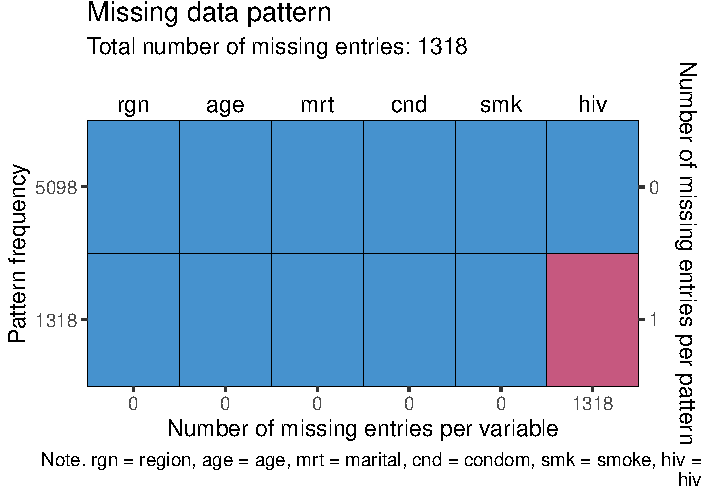
\includegraphics{Manuscript_files/figure-latex/hiv-1} \end{center}

\end{CodeChunk}

From the missing data pattern we see that we can set \texttt{maxit} to
1, since there is only one variable with missingness.

The inclusion restriction variable should be a predictor of the the
actual value of the variable of interest, but \emph{not} of missingness
indicator for the variable of interest. In this case, the data were
simulated to adhere to this requirement. Namely, \(\beta_{smoke}\) =
-0.064, 95\% CI {[}-0.256, 0.126{]} for the analysis model
(\texttt{formula\ =\ hiv\ \textasciitilde{}\ .}), and \(\beta_{smoke}\)
= -0.265, 95\% CI {[}-0.422, -0.11{]} for the selection model
(\texttt{formula\ =\ is.na(hiv)\ \textasciitilde{}\ .}). This means the
assumptions for the Heckman-type selection model are met.

\hypertarget{how-to-handle-multivariate-missingness-case-study-iii-impact}{%
\section{How to handle multivariate missingness (Case study III:
IMPACT)}\label{how-to-handle-multivariate-missingness-case-study-iii-impact}}

\texttt{impact} is traumatic brain injury data with patients,
\(n = 11022\), clustered in studies, \(N = 15\). With the following 11
variables:

\begin{itemize}
\tightlist
\item
  \texttt{name} Name of the study,
\item
  \texttt{type} Type of study (RCT: randomized controlled trial, OBS:
  observational cohort),
\item
  \texttt{age} Age of the patient,
\item
  \texttt{motor\_score} Glasgow Coma Scale motor score,
\item
  \texttt{pupil} Pupillary reactivity,
\item
  \texttt{ct} Marshall Computerized Tomography classification,
\item
  \texttt{hypox} Hypoxia (0=no, 1=yes),
\item
  \texttt{hypots} Hypotension (0=no, 1=yes),
\item
  \texttt{tsah} Traumatic subarachnoid hemorrhage (0=no, 1=yes),
\item
  \texttt{edh} Epidural hematoma (0=no, 1=yes),
\item
  \texttt{mort} 6-month mortality (0=alive, 1=dead).
\end{itemize}

The data is already imputed (Steyerberg et al, 2008), so we'll induce
missingness ourselves. For example, MAR missingness varying by
cluster.\footnote{Observed data pattern should differ per cluster. So,
  in cluster 1, the missingness would depend on age, but not in cluster
  two. Split the dataframe and run \texttt{ampute()} on each cluster.}

\begin{CodeChunk}


\begin{center}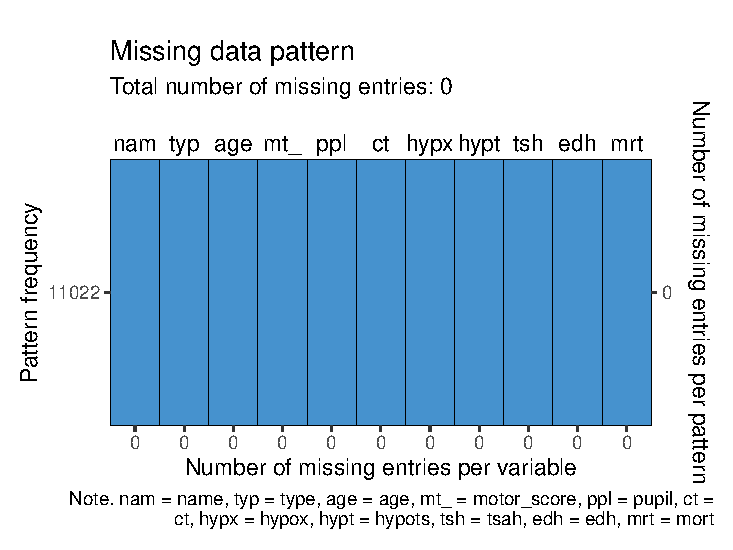
\includegraphics{Manuscript_files/figure-latex/impact-1} \end{center}



\begin{center}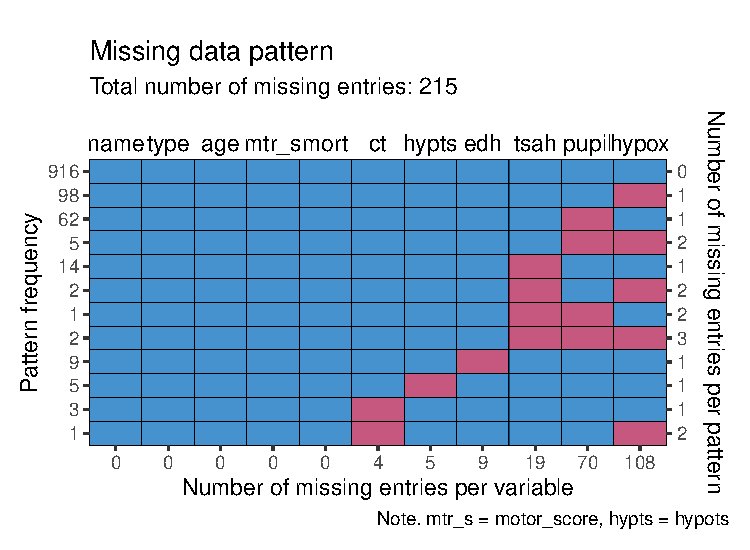
\includegraphics{Manuscript_files/figure-latex/impact-2} \end{center}



\begin{center}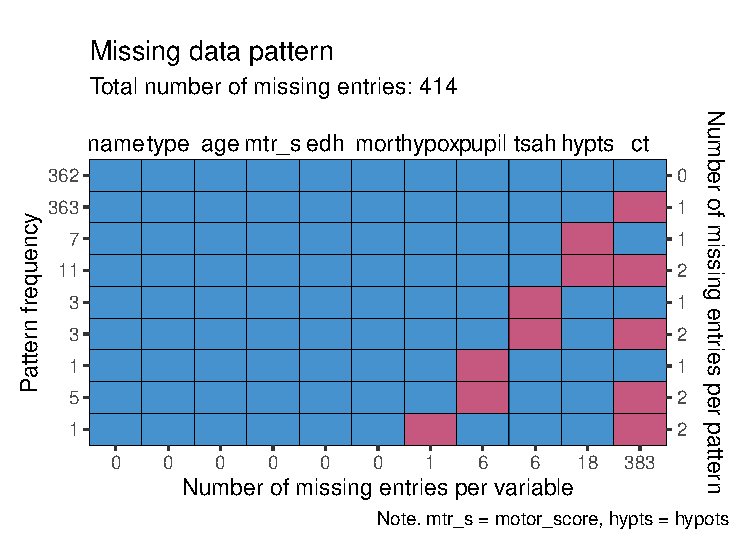
\includegraphics{Manuscript_files/figure-latex/impact-3} \end{center}

\end{CodeChunk}

\hypertarget{discussion}{%
\section{Discussion}\label{discussion}}

\begin{itemize}
\item
  JOMO in \pkg{mice} -\textgreater{} on the side for now
\item
  Additional levels of clustering
\item
  More complex data types: timeseries and polynomial relationship in the
  clustering.
\end{itemize}

\hypertarget{think-about}{%
\section{Think about}\label{think-about}}

\begin{itemize}
\item
  Adding some kind of help function to mice that suggests a suitable
  predictor matrix to the user, given a certain analysis model.
\item
  Adding a \texttt{multilevel\_ampute()} wrapper function in mice.
\item
  Exporting \texttt{mids} objects to other packages like \texttt{lme4}
  or \texttt{coxme}?
\item
  Adding a ICC=0 dataset to show that even if there is no clustering it
  doesn't hurt.
\end{itemize}

\renewcommand\refname{References}
\bibliography{../References/multilevelmice.bib}



\end{document}
